\label{Effective potential}
\subsection{QFT via path integrals}
This section is based on \cite{Peskin:IntroQFT,weinberg_1995,weinberg_1996_vol2} (Schwarz).
The ground state path integral is given by
\begin{equation}
    Z = \lim_{T\rightarrow \infty} \braket{\Omega, T}{-T, \Omega}
    = \lim_{T\rightarrow \infty} \inner{\Omega}{ e^{-2iHT} }{\Omega}
    = \int \D \pi \D \varphi \, \exp{ i \int \dd^4 x \, \left(\pi \dot \varphi - \He[\pi, \varphi]\right) },
\end{equation}
where $\ket{\Omega}$ is the vacuum of the theory~\cite{Peskin:IntroQFT,weinberg_1995}.
By introducing a source term into the Hamiltonian, $\He \rightarrow \He - J(x)\varphi(x)$, we get the generating functional
\begin{equation}
    Z[J] = 
    \int \D \pi \D \varphi \, 
    \exp{ i \int \dd^4 x \, \left(\pi \dot \varphi - \He[\pi, \varphi]+ J\varphi\right) }
\end{equation}
If $\He$ is quadratic in $\pi$, we can complete the square and integrate out $\pi$ to obtain
\begin{equation}
    Z[J] = C \int \D \varphi \, \exp{i \int \dd^4 x\, (\Ell[\varphi] + J \varphi)}.
\end{equation}
$C$ is infinite, but constant, and will drop out of physical quantities.
$Z[J]$ is called the generating functional as correlation functions $\ex{\varphi(X_1)\varphi(X_2)...} = \inner{\Omega}{T{\varphi(X_1)\varphi(X_2)\dots}}{\Omega}$ are given by functional derivatives of $Z[J]$, 
\begin{equation}
    \label{correlator from generating functional}
    \ex{\varphi(X_1)\varphi(X_2)...}
    = 
    \frac{\int \D \varphi(X)\,  (\varphi(X_1)\varphi(X_2)...) e^{i S[\varphi]}}
        {\int \D \varphi(X)\, e^{i S[\varphi]}}
    =
    \frac{1}{Z[0]} \prod_i\left( -i  \fdv{J(X_i)}\right) Z[J]\Big|_{J = 0},
\end{equation}
where 
\begin{equation}
    S[\varphi] = \int \dd^4 x \, \Ell[\varphi]
\end{equation}
is the action.
The functional derivative is described in \autoref{section:Functional derivative}.

% By Wick's theorem, an $n$-point correlated is given by the sum of all Feynman diagrams with $n$ external vertices.
% The factor $Z[0]^{-1}$ divides out all \emph{vacuum bubbles}, that is diagrams without external vertices.
% We can show this by considering 

In a free theory, we are able to write
\begin{equation}
    Z_0[J] = Z_0[0] \exp(i W_0[J]), \quad 
    W_0[J] = \frac{1}{2} \int \dd^4 x \dd^4 y \, J(x) D_0(x - y) J(y),
\end{equation}
where $D_0$ is the propagator of the free theory.
The exponential form of $Z[J]$ leads to Wick's theorem, which states that an expectation value of $2n$ fields is a sum of \emph{all possible, distinct} combination of $n$ propagators.
To write this in a formal way, we define the functions $a$ and $b$, which define a way to pair up $2m$ elements.
The domain of the functions are the integers between $1$ and $m$, the image a subset of the integers between $1$ and $2m$ of size $m$.
A valid pairing is a set $\{(a(1), b(1)), \dots (a(m), b(m))\}$, where all elements $a(i)$ and $b(j)$ are different, such all integers up to and including $2m$ are featured.
A pair is not directed, so $(a(i), b(i))$ is the same pair as $(b(i), a(i))$.
Wick theorem states that,
\begin{equation}
    \ex{{\prod}_{i=1}^{2m} \varphi(x_i)  }_0
    = \sum_{\{(a, b)\}} \ex{\varphi(x_{a(i)}) \varphi(x_{b(i)})}_0,
\end{equation}
where the sum is over all tuples $(a, b)$ that define a valid and unique pairing.
A generating functional in a general theory is 
\begin{equation}
    Z[J] 
    = Z[0] \ex{\exp(iS_I + i\int \dd^4 x \, J(x) \varphi(x))}_0,
\end{equation}
where the subscript indicates that the expectation value is taken in the free theory.
The expectation value can be expanded in a power series, 
\begin{equation}
    \sum_{n, m} \frac{1}{n! m!} \ex{(iS_I)^n \left(i\int \dd^4 x \, J(x) \varphi(x)\right)^m}_0.
\end{equation}
This equals \emph{the sum of all diagrams with external sources $J(x)$}.
The expectation value
\begin{equation}
    \ex{(iS_I)^n (\varphi(x)J(x))^m}_0
\end{equation}
are all diagrams with $n$ vertices given by the Feynman rules from the interacting action $S_I$, as well as $m$ m source vertices.

Consider a general diagram, built up of $N$ different connected sub-diagrams, where sub-diagram $i$ appears $n_i$ times.
As an illustration, a generic vacuum diagram in $\phi^4$-theory has the form
\begin{align}
    \label{Feinman diagrams}
    V = 
    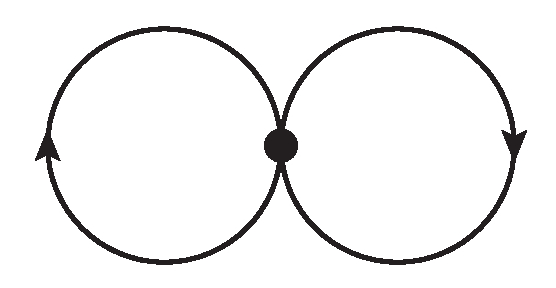
\includegraphics[width=0.1\textwidth, valign=c]{figurer/feynman-diagram/phi-4_loop_notext.eps}
    \times
    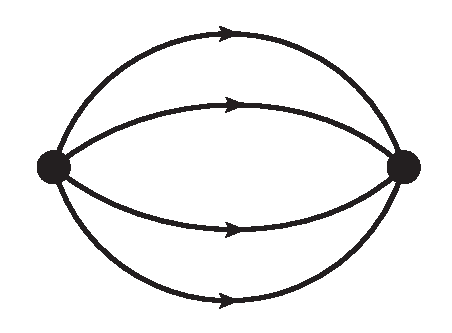
\includegraphics[width=0.08\textwidth, valign=c]{figurer/feynman-diagram/phi-4_2_loop.eps}
    \times
    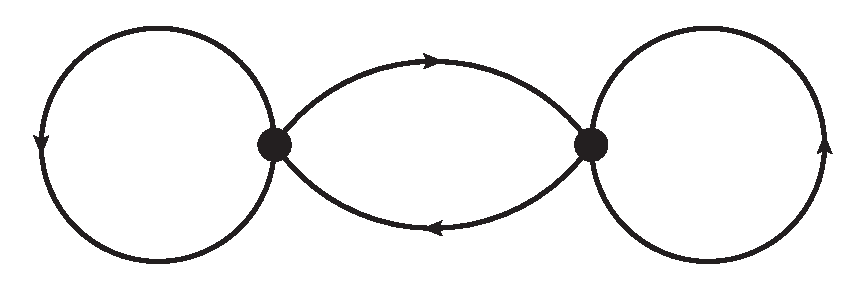
\includegraphics[width=0.14\textwidth, valign=c]{figurer/feynman-diagram/phi-4_2_loop2.eps}
    \times
    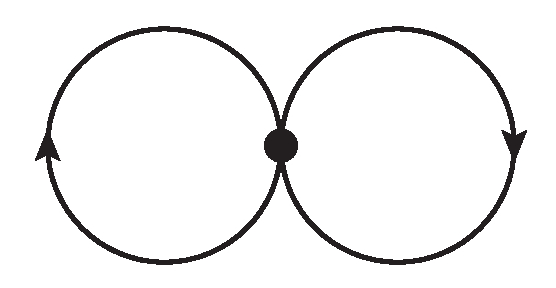
\includegraphics[width=0.1\textwidth, valign=c]{figurer/feynman-diagram/phi-4_loop_notext.eps}
    \times \dots.
\end{align}
If the value of sub diagram $i$ is $V_i$, then each copy of that sub diagram contribute a factor $V_i$ to the value of the total diagram.
However, due to the symmetry of permuting identical sub diagrams, one must divide by the extra symmetry factor $s = n_i !$, which is the total number of permutation of all the copies of diagram $i$.
The value of the total diagram is therefore
\begin{align}
    \label{Feynman diagrams}
    V
    = \prod_{i= 1}^N \frac{1}{n_i!} V_i^{n_i}.
\end{align}
$V$ is uniquely defined by a finite sequence of integers, $(n_1, n_2, \dots n_N, 0, 0, \dots)$, so the sum of all diagrams is the sum over the set $S$ of all finite integers.
This allows us to write the sum of all diagrams as
\begin{equation}
    \label{sum of all diagrams}
    \sum_{(n_1, ...)\in S} \prod_{i} \frac{1}{n_i!} V_i^{n_i}
    = \prod_{i = 1}^{\infty} \sum_{n_i=1}^{\infty} \frac{1}{n_i!} V_i^{n_i}
    = \exp(i {\sum}_i V_i).
\end{equation}
We showed that the generating functional $Z[J]$ were the sum of all diagrams due to external currents.
Using \autoref{sum of all diagrams}, we see that the sum of all \emph{connected} diagrams $W[J]$ is given by
\begin{equation}
    Z[J] = Z[0]\exp(i W[J]).
\end{equation}
We can see that this is trivially true for the free theory, the only connected diagram is
\begin{equation}
    W_0[J] = 
    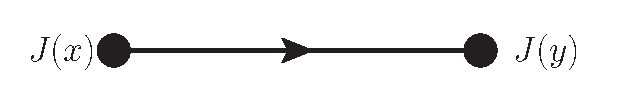
\includegraphics[valign=c, width=0.3\textwidth]{figurer/feynman-diagram/current-current.eps}.
\end{equation}
Furthermore, correlation functions in the full interacting theory is
\begin{equation}
    \label{correlation function}
    \ex{\varphi(x_1)\dots} = \left(\prod_i \funcdv{J(x_i)}\right) W[J] \Big|_{J=0}.
\end{equation}

% Here we defined the \emph{generating functional for connected diagrams}, $W[J]$.
% The reason for the name will become apparent later. (HUSK Å REFFERE TILBAKE)
% The expectation value of some function of the field-configuration, $A = A[\varphi]$, in the precesense of the source $J$ is
% \begin{equation}
%     \ex{A}_J = \frac{1}{Z[J]} A\left( -i  \fdv{J}\right) Z[J].
% \end{equation}
% (DEFINE FUNCTIONAL DERIVATIVE)
% The expectation value of the field defines a functional,
% \begin{equation}
%     \label{calssical field functional}
%     \varphi[J](x) = \ex{\varphi(x)}_J = 
%     \frac{1}{Z[J]} \left( -i  \fdv{J}\right) Z[J]
%     = \fdv{J(x)} W[J],
% \end{equation}
% and is sometimes called the \emph{classical field}.
% The notation $\Ef[f](x)$ means that $\Ef$ is a functional which takes in a function $f$, and returns the new function $(\Ef[f])(x)$.
% One example is the Lagrangian density, which takes in a field, and returns a function which has a value for each point in space-time.
% We can reverse this relationship, by defining the functional $J[\varphi](x)$ as \emph{the current which causes the classical field $\varphi$}.
% That is, if $\varphi[J_0](x) = \varphi_0(x)$ for some source $J_0$, then $J[\varphi_0] = J_0$
